%%%%%%%%%%%%%%%%%%%%%%%%%%%%%%%%%%%%%%%%%%%%%%%%%%%%%%%%%%%%%%%%%%%%%%%%%%%%%%%%
\chapter{Реализация алгоритма извлечения вопросно-ответных пар}
\label{chap:impl}
%%%%%%%%%%%%%%%%%%%%%%%%%%%%%%%%%%%%%%%%%%%%%%%%%%%%%%%%%%%%%%%%%%%%%%%%%%%%%%%%

Для оценки эффективности предложенного в разделе~\ref{chap:dev} решения, реализуем его в виде программной библиотеки (реализация алгоритма). Результаты, полученные с помощью данной реализации будут использованы в разделе~\ref{chap:quality} для проведения экспертного анализа и при оценке эффективности решения.

В данном разделе рассматриваются некоторые аспекты реализации преложенного метода извлечения ВОП из обращений в службу поддержки, описана структура проекта, определены используемые технологии. Полный текст реализации алгоритма доступен на прилагаемом к данной работе CD-диске.

%%%%%%%%%%%%%%%%%%%%%%%%%%%%%%%%%%%%%%%%%%%%%%%%%%%%%%%%%%%%%%%%%%%%%%%%%%%%%%%%
\section{Используемые технологии}
%%%%%%%%%%%%%%%%%%%%%%%%%%%%%%%%%%%%%%%%%%%%%%%%%%%%%%%%%%%%%%%%%%%%%%%%%%%%%%%%
При реализации алгоритма использовались следующие технологии: Java, Kotlin, Gradle, Git, JUnit, MongoDB, Mallet.

В качестве языка программирования используется \textit{Kotlin}. Kotlin~--- это активно развивающийся язык программирования общего назначения для JVM, к достоинствам которого относятся:

\nomenclature{JVM}{Java Virtual Machine, виртуальная машина java}

\begin{itemize*}
\item Вывод типов;
\item Статическая типизация;
\item Мультипарадигменность;
\item Nullable типы данных;
\item Выразительный синтаксис;
\item Совместимость с java кодом.
\end{itemize*}

Описанные выше достоинства языка позволяют решать поставленные перед программистом задачи более эффективно, чем при использовании java. При этом, благодаря совместимости с java, сохраняется возможность использования большого количества существующих java-библиотек.

На момент написания данной работы, Kotlin поддерживает Gradle, Maven и Ant для автоматической сборки проектов. \textit{Gradle}~--- система автоматической сборки, предоставляющая DSL на языке Groovy, и, по сравнению с другими решениями, использующими XML, позволяет писать более компактные сценарии сборки.

\nomenclature{DSL}{Domain-Specific Language, предметно-ориентированный язык}
\nomenclature{XML}{eXtensible Markup Language, расширяемый язык разметки}
\nomenclature{JSON}{JavaScript Object Notation, синтаксис для описания объектов и данных}
\nomenclature{СУБД}{Система Управления Базами Данных}

\textit{Git}~--- система контроля версий, используемая командой YouTrack.

\textit{JUnit}~--- библиотека для модульного тестирования программного обеспечения. Совместима с Kotlin.

Для хранения данных используется \textit{MongoDB}. Для работы с обращениями в службу поддержки команда YouTrack использует Zendesk. Загружаемые из Zendesk данные имеют JSON формат. Поскольку MongoDB использует JSON-подобные документы и схему базы данных, было решено использовать данную СУБД, вместо реляционных баз данных.

\textit{Mallet}~\cite{MALLET}~--- библиотека на java, которая содержит реализацию необходимой тематической модели (LDA). Данная реализация написана в 2009 году, является наиболее \quotes{взрослой} и развитой реализацией LDA. Подробнее о выборе реализации LDA написано в секции~\ref{sec:lda_choose}.

%%%%%%%%%%%%%%%%%%%%%%%%%%%%%%%%%%%%%%%%%%%%%%%%%%%%%%%%%%%%%%%%%%%%%%%%%%%%%%%%
\section{Структура проекта}
%%%%%%%%%%%%%%%%%%%%%%%%%%%%%%%%%%%%%%%%%%%%%%%%%%%%%%%%%%%%%%%%%%%%%%%%%%%%%%%%

Структура проекта представляет собой набор пакетов (\textit{packages}). Общая структура пакетов представлена на рисунке~\ref{fig:pckgs}. 

\begin{figure}[tph!]
\centerline{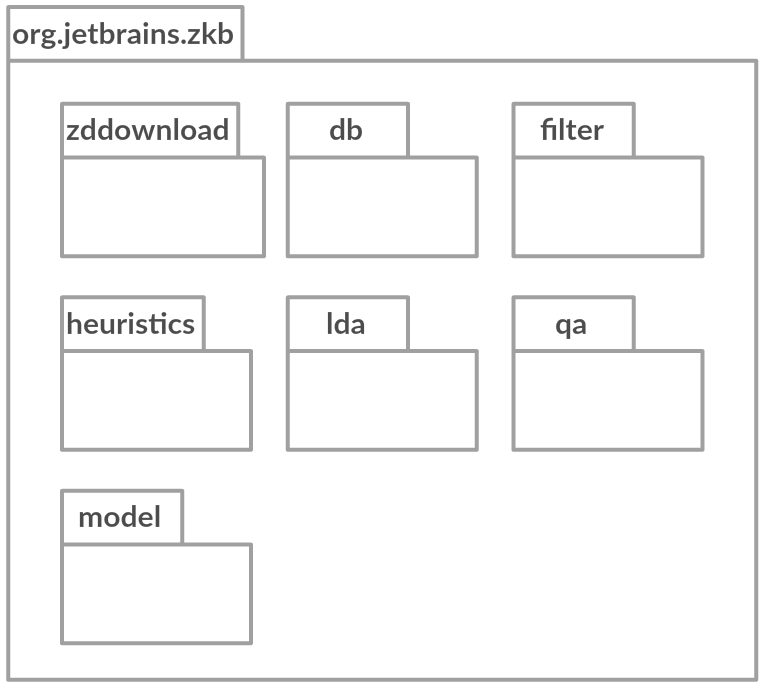
\includegraphics[width=7.5cm]{fig/pckgs.png}}
    \caption{Обобщенная структура пакетов реализации алгоритма}
    \label{fig:pckgs}
\end{figure}

Каждый из пакетов выполняет соответсвующую ему задачу:

\begin{itemize*}
\item org.jetbrains.zkb.zddownload~--- загрузка данных из Zendesk и сохранение их в базу данных;
\item org.jetbrains.zkb.model~--- модель данных, классы Comment (комментарий), QAPair (пара вопрос-ответ) и так далее.
\item org.jetbrains.zkb.db~--- данный пакет содержит классы отвечающие за взаимодействие с базой данных;
\item org.jetbrains.zkb.filter~--- содержит фильтры различного рода для анализируемых данных;
\item org.jetbrains.zkb.heuristics~--- эвристики предобработки;
\item org.jetbrains.zkb.lda~--- построение тематической модели анализируемых данных;
\item org.jetbrains.zkb.qa~--- формирование ВОП;

\end{itemize*}

Далее каждый из пакетов рассматривается более подробно.

%%%%%%%%%%%%%%%%%%%%%%%%%%%%%%%%%%%%%%%%%%%%%%%%%%%%%%%%%%%%%%%%%%%%%%%%%%%%%%%%
\section{Получение исходных данных}
\label{sec:zddwn}
%%%%%%%%%%%%%%%%%%%%%%%%%%%%%%%%%%%%%%%%%%%%%%%%%%%%%%%%%%%%%%%%%%%%%%%%%%%%%%%%

Пакет \textbf{org.jetbrains.zkb.zddownload} содержит программный код отвечающий за загрузку данных из Zendesk.

Взаимодействие с Zendesk происходит через REST API~\cite{zdapi}. В Zendesk обращение представлено такой сущностью, как \quotes{Ticket} (тикет). Тикет содержит ряд метаинформации об обращении: уникальный идентификатор обращения, дата и время создания, дата и время последнего обновления, статус обращения, уникальный идентификатор инициатора и так далее~--- однако информация о соответствующих данному обращению комментариях отсутствует.

\nomenclature{REST}{Representational State Transfer, передача состояния представления}
\nomenclature{API}{Application Programming Interface, программный интерфейс приложения}

Комментарии представлены сущностью \quotes{Comment}, содержащей текст комментария и также некоторую дополнительную метаинформацию: уникальные идентификаторы комментария и автора, дата и время создания и так далее. Таким образом, для получения достаточной для дальней обработки информации об одном обращении, необходимо загрузить:

\begin{enumerate*}
\item Объект представляющий обращение (Ticket);
\item Все комментарии (Comment), принадлежащее данному обращению;
\end{enumerate*}

Для загрузки данных использовался клиент\footnote{https://github.com/cloudbees/zendesk-java-client \label{fn:zdcl}} для Zendesk API с открытым исходным кодом. Важным ограничением, которое нужно учитывать при взаимодействии с Zendesk~--- это ограничение на количество запросов в минуту. При интенсивном использовании API Zendesk может заблокировать все входящие запросы на некоторое время. Чтобы избежать данной ситуации, клиент$^{\ref{fn:zdcl}}$ был модифицирован. Был добавлен учёт оставшегося количества запросов, а также интервал между запросами. Соответствующий фрагмент программы приведен ниже (листинг~\ref{listings:zddwnld}):

\lstinputlisting[
  label={listings:zddwnld},
  caption={Ограничение на исползование Zendesk API},
  style={java}
]
{code/Zendesk.java}

В листинге~\ref{listings:zddwnld2} приведен текст функции, отвечающей за загрузку данных из Zendesk. Частично загруженная информация сохраняется в базу данных (функция \textit{saveData()}) во избежание потери при разрыве соединения.

\lstinputlisting[
  linerange={50-83},
  label={listings:zddwnld2},
  caption={Загрузка данных из Zendesk},
  style={java}
]
{code/getData.kt}

\lstinputlisting[
  linerange={146-146},
  label={listings:zddwnld3},
  caption={Объявление функции \textit{wrapZendeskAPICall()}},
  style={java}
]
{code/getData.kt}

Все обращения к API происходят внутри функции \textit{wrapZendeskAPICall()} (листинг~\ref{listings:zddwnld3}), задача которой~--- корректная обработка исключительных ситуаций, возможных при обращении к Zendesk API.

%%%%%%%%%%%%%%%%%%%%%%%%%%%%%%%%%%%%%%%%%%%%%%%%%%%%%%%%%%%%%%%%%%%%%%%%%%%%%%%%
\section{Модель данных}
%%%%%%%%%%%%%%%%%%%%%%%%%%%%%%%%%%%%%%%%%%%%%%%%%%%%%%%%%%%%%%%%%%%%%%%%%%%%%%%%

Классы модели данных находятся в пакете \textbf{org.jetbrains.zkb.model}. Соответствующая диаграмма классов приведена на рисунке~\ref{fig:umodel}. Класс \textit{Ticket} располагается вне данного пакета, вместо реализации данного класса используется модель, предоставляемая клиентом Zendesk (секция~\ref{sec:zddwn}).

\begin{figure}[tph!]
\centerline{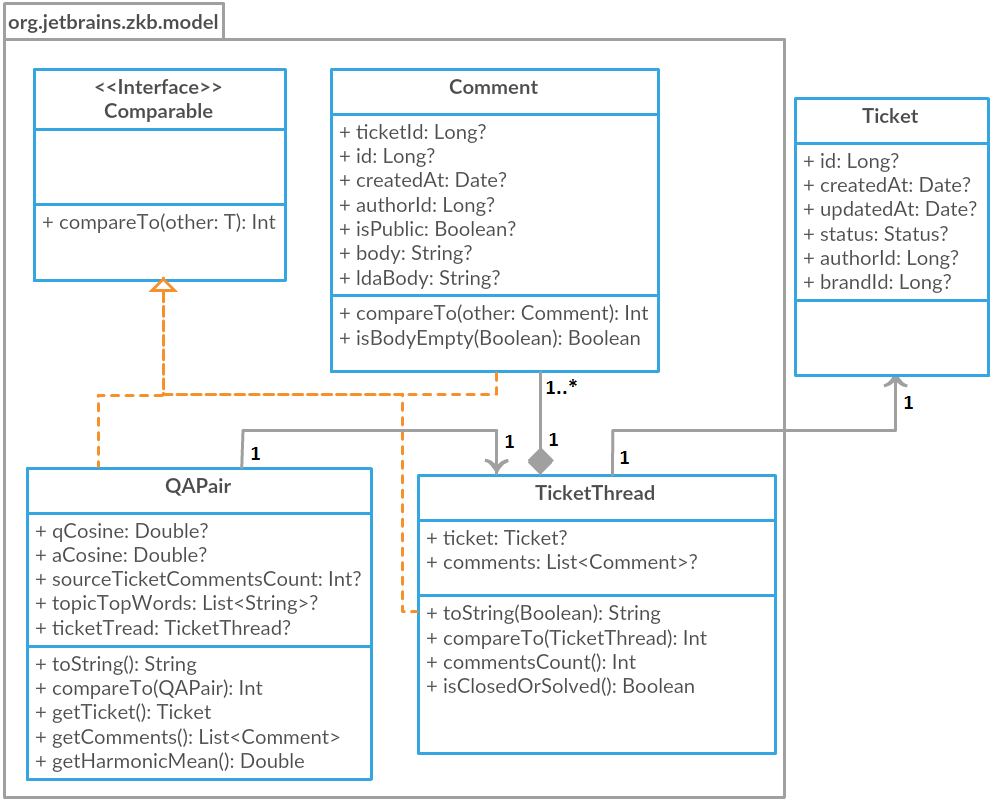
\includegraphics[width=11cm]{fig/model.png}}
    \caption{Диаграмма классов пакета org.jetbrains.zkb.model}
    \label{fig:umodel}
\end{figure}

Каждый из приведенных на рисунке~\ref{fig:umodel} классов поддерживает сериализацию в формат JSON. Поддержка сериализации объектов необходима для организации взаимодействия с Zendesk и MongoDB. Для этого использовалась библиотека Jackson\footnote{https://github.com/FasterXML/jackson} с добавлением к классам специальных аннотаций. В листинге~\ref{listings:comment} приведен пример класса \textit{Comment} c соответствующими аннотациями.

\lstinputlisting[
  label={listings:comment},
  caption={Пример использования библиотеки Jackson},
  style={java}
]
{code/Comment.kt}

%%%%%%%%%%%%%%%%%%%%%%%%%%%%%%%%%%%%%%%%%%%%%%%%%%%%%%%%%%%%%%%%%%%%%%%%%%%%%%%%
\section{Взаимодействие с базой данных}
%%%%%%%%%%%%%%%%%%%%%%%%%%%%%%%%%%%%%%%%%%%%%%%%%%%%%%%%%%%%%%%%%%%%%%%%%%%%%%%%

Логика взаимодействия базой данных инкапсулирована в классах \textit{DBReader} и \textit{DBWriter}, которые располагаются в пакете \textbf{org.jetbrains.zkb.db}. Диаграмма классов данного пакета приведена на рисунке~\ref{fig:dbdmodel}.

\begin{figure}[tph!]
\centerline{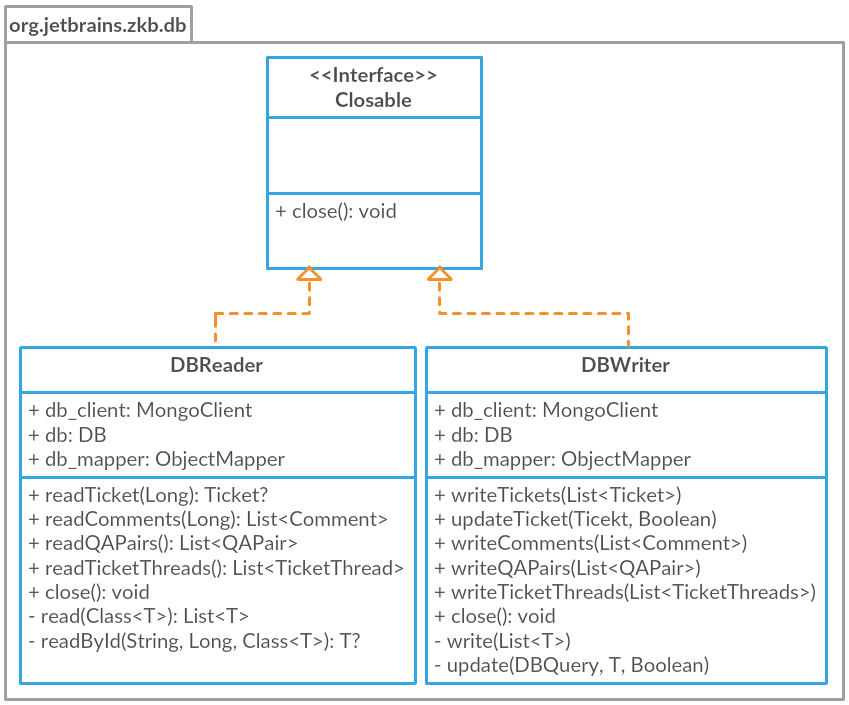
\includegraphics[width=9cm]{fig/dbmodel.png}}
    \caption{Диаграмма классов пакета org.jetbrains.zkb.db}
    \label{fig:dbdmodel}
\end{figure}

\nomenclature{BSON}{Binary JavaScript Object Notation, формат электронного обмена цифровыми данными, основанный на JavaScript}

MongoDB для хранения данных использует формат BSON. Класс \textit{DBReader} реализует логику трансформации объектов в JSON формат, который затем преобразуется в BSON и сохраняется в базу данных. Класс \textit{DBWriter} позволяет читать данные из базы данных, преобразуя их из BSON формата к объектам Kotlin.

%%%%%%%%%%%%%%%%%%%%%%%%%%%%%%%%%%%%%%%%%%%%%%%%%%%%%%%%%%%%%%%%%%%%%%%%%%%%%%%%
\section{Реализация предобработки данных}
%%%%%%%%%%%%%%%%%%%%%%%%%%%%%%%%%%%%%%%%%%%%%%%%%%%%%%%%%%%%%%%%%%%%%%%%%%%%%%%%
\subsection{Фильтрация данных}
За фильтрацию данных отвечает пакет \textbf{org.jetbrains.zkb.filter}. Фильтры представлены в виде набора функций, применяемых к коллекции фильтруемых объектов и возвращающих элементы, прошедшие фильтрацию. Эти фильтрующие функции поделены по файлам в соответствии с типом данных, к которым они применяются.

\begin{itemize*}
\item \textit{comments.kt}~--- удаление дубликатов; фильтрация комментариев для определенного набора обращений; фильтрация не пустых комментариев (после применения эвристик) и так далее;
\item \textit{tickets.kt}~--- фильтрация обращений с определенным статусом; удаление дубликатов; фильтрация обращений, относящихся к YouTrack;
\item \textit{ticketThreads.kt}~--- фильтр обращений с определенным количеством комментариев; фильтр обращений на английском языке и так далее;
\item \textit{filterData.kt}~--- применение описанных ранее функций фильтрации к необработанным данным.
\end{itemize*}

Структура данного пакета показана на рисунке~\ref{fig:filterpck}.

\begin{figure}[tph!]
\centerline{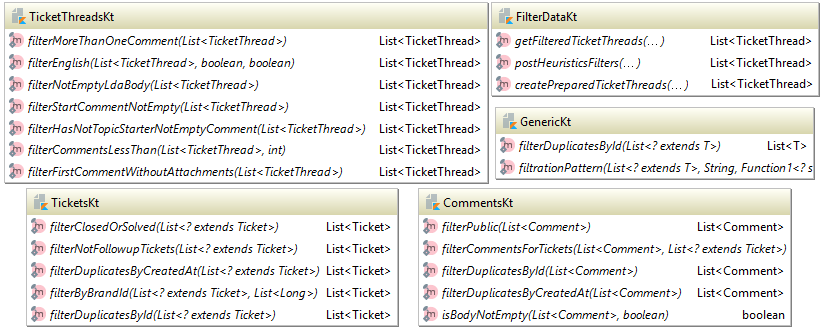
\includegraphics[width=11cm]{fig/filterpck.png}}
    \caption{Структура пакета org.jetbrains.zkb.filter}
    \label{fig:filterpck}
\end{figure}

\subsection{Эвристики предобработки}

Пакет \textbf{org.jetbrains.zkb.heuristics} содержит реализацию эвристик предобработки. Данный пакет реализован аналогично пакету, содержащему фильтрующие функции~--- эвристики предобработки представлены в виде функций, разделенных по файлам в соответствии с типом данных к которым они применяются.

\begin{itemize*}
\item \textit{comments.kt}~--- содержит реализацию эвристик, описанных в разделе~\ref{chap:dev};
\item \textit{ticketThreads.kt}~--- представляет API применения эвристик предобработки для коллекции \textit{TicketThreads}. Содержит функцию \textit{applyHeurisitics()}, агрегирующую применение всех эвристик.
\end{itemize*}

Реализация функции \textit{applyHeurisitics()} приведена в листинге~\ref{listings:heur}.

\lstinputlisting[
  label={listings:heur},
  caption={Применение эвристик предобработки данных},
  style={java}
]
{code/ttHeur.kt}

%%%%%%%%%%%%%%%%%%%%%%%%%%%%%%%%%%%%%%%%%%%%%%%%%%%%%%%%%%%%%%%%%%%%%%%%%%%%%%%%
\section{Построение тематической модели}
%%%%%%%%%%%%%%%%%%%%%%%%%%%%%%%%%%%%%%%%%%%%%%%%%%%%%%%%%%%%%%%%%%%%%%%%%%%%%%%%
\subsection{Выбор реализации LDA}
\label{sec:lda_choose}

В данной работе используется реализация LDA, содержащаяся в библиотеке MALLET~\cite{MALLET}.

MALLET~--- библиотека на java, применяющаяся для анализа текста, классификации документов, тематического моделирования и так далее. Разработана Эндрю МакКаллум в университете города Амхерст (UMass Amherst) в 2002 году.  Реализация LDA была добавлена в эту библиотеку в 2009 году. Данная реализация является наиболее \quotes{взрослой} и развитой реализацией LDA, в том числе используется авторами работы~\cite{original}.

В 2015 году была добавлена реализация LDA в библиотеку \mbox{scikit-learn}~\cite{scikit-learn-lda}, написанную на языке python. Использование данной реализации привело бы к необходимости организации дополнительного взаимодействия между Kotlin и python, что усложнило бы процесс разработки.

Другие java-реализации LDA:
\begin{itemize}
\item LDA in Mahout\footnote{https://mahout.apache.org/users/clustering/latent-dirichlet-allocation.html}~--- используется map-reduce подход, что применимо для больших данных и неактуально для данной работы;
\item LDA in Spark\footnote{https://spark.apache.org/docs/latest/mllib-clustering.html}~--- в документации указано, что данная реализация LDA является экспериментальной, в связи с чем нет уверенности в её стабильности;
\item jLDADMM\footnote{http://jldadmm.sourceforge.net/}~--- специфичная реализация для анализа коротких текстов.
\end{itemize}

\subsection{Пакет org.jetbrains.zkb.lda}

Структура данного пакета приведена на рисунке~\ref{fig:lda}.

\begin{figure}[tph!]
\centerline{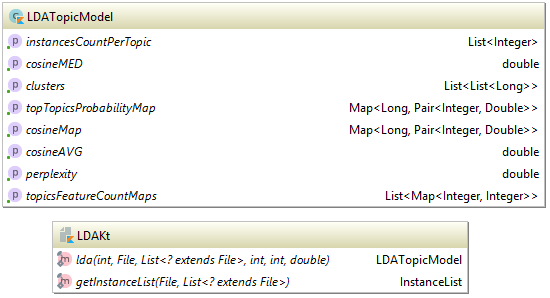
\includegraphics[width=11cm]{fig/lda.png}}
    \caption{Структура пакета org.jetbrains.zkb.lda}
    \label{fig:lda}
\end{figure}

Класс \textit{LDATopicModel} наследуется от класса ParallelTopicModel, предоставляемого библиотекой MALLET и реализующего модель LDA, добавляет функциональность по вычислению перплексии полученной модели, построению кластеров обращений на основе темы с наибольшей вероятностью и некоторую другую. В листинге~\ref{listings:ldaTM} представлен упрощенный код класса \textit{LDATopicModel} без детальной реализации.

\lstinputlisting[
  label={listings:ldaTM},
  caption={Класс LDATopicModel},
  style={java}
]
{code/ldaTM.kt}

За создание и обучение тематической модели отвечает функция \textit{lda()}, программный код которой приведен в листинге~\ref{listings:lda}.

\lstinputlisting[
  label={listings:lda},
  caption={Создание и обучение тематической модели},
  style={java}
]
{code/lda.kt}

%%%%%%%%%%%%%%%%%%%%%%%%%%%%%%%%%%%%%%%%%%%%%%%%%%%%%%%%%%%%%%%%%%%%%%%%%%%%%%%%
\section{Поиск вопросно-ответных пар}
%%%%%%%%%%%%%%%%%%%%%%%%%%%%%%%%%%%%%%%%%%%%%%%%%%%%%%%%%%%%%%%%%%%%%%%%%%%%%%%%
Программный код, решающий задачу поиска ВОП расположен в пакете \textbf{org.jetbrains.zkb.qa}, структуру которого можно увидеть на рисунке~\ref{fig:qapck}.

\begin{figure}[tph!]
\centerline{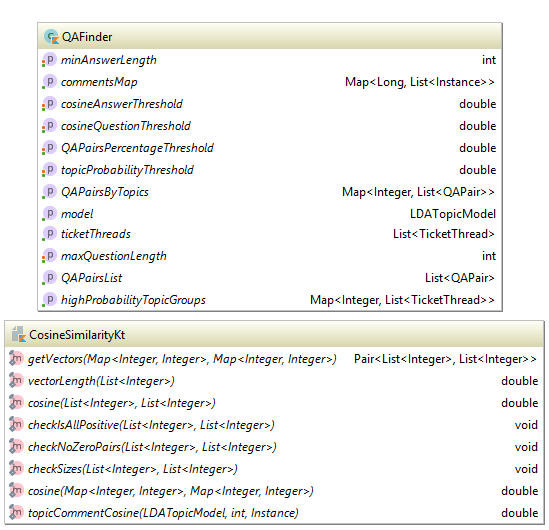
\includegraphics[width=11cm]{fig/qapck.png}}
    \caption{Структура пакета org.jetbrains.zkb.lda}
    \label{fig:qapck}
\end{figure}

Класс \textit{QAFinder} инкапсулирует логику, описанную в секции~\ref{sec:qaforming}. Его основными методами для публичного использования являются:

\begin{itemize}
\item \textit{getQAPairsList()}~--- возвращает отсортированный в порядке уменьшения значения гармонического среднего список объектов \textit{QAPair};
\item \textit{getQAPairsByTopics()}~--- возвращает коллекцию списков объектов \textit{QAPair}, где каждый список содержит ВОП, принадлежащие к одной теме.
\end{itemize}

Расчет косинусного расстояние вынесен за пределы класса \textit{QAFinder} поскольку помимо этого класса функция расчета косинуса используется в классе \textit{LDATopicModel}. 

Функция \textit{getVectors()} вычисляет векторы, соответствующие текстам, между которыми необходимо посчитать расстояние (листинг~\ref{listings:vectors}). Результат данной функции затем передается в функцию \textit{cosine()} для определения косинускного расстояния (листинг~\ref{listings:cos}).

\lstinputlisting[
  linerange={9-37},
  label={listings:vectors},
  caption={Построение векторов},
  style={java}
]
{code/cosineSimilarity.kt}

\lstinputlisting[
  linerange={42-51},
  label={listings:cos},
  caption={Вычисление косинусного расстояния},
  style={java}
]
{code/cosineSimilarity.kt}

%%%%%%%%%%%%%%%%%%%%%%%%%%%%%%%%%%%%%%%%%%%%%%%%%%%%%%%%%%%%%%%%%%%%%%%%%%%%%%%%
\section{Резюме}
%%%%%%%%%%%%%%%%%%%%%%%%%%%%%%%%%%%%%%%%%%%%%%%%%%%%%%%%%%%%%%%%%%%%%%%%%%%%%%%%

В данном разделе рассмотрены основные аспекты реализации преложенного метода извлечения ВОП из обращений в службу поддержки. Описаны используемые технологии, структура проекта. Приведены листинги некоторых функций и классов, UML-диаграммы классов соответствующих пакетов.
